\documentclass[11pt]{article}
\usepackage{euscript}

\usepackage{amsmath}
\usepackage{amsthm}
\usepackage{amssymb}
\usepackage{mathtools}
\DeclarePairedDelimiter{\ceil}{\lceil}{\rceil}
\usepackage{epsfig}
\usepackage{xspace}
\usepackage{color}
\usepackage{url}
\usepackage{enumerate}
\usepackage{listings}

\usepackage{float}

%%%%%%%  For drawing trees  %%%%%%%%%
\usepackage{tikz}
\usetikzlibrary{calc, shapes, backgrounds}

%%%%%%%%%%%%%%%%%%%%%%%%%%%%%%%%%
\setlength{\textheight}{9in}
\setlength{\topmargin}{-0.600in}
\setlength{\headheight}{0.2in}
\setlength{\headsep}{0.250in}
\setlength{\footskip}{0.5in}
\flushbottom
\setlength{\textwidth}{6.5in}
\setlength{\oddsidemargin}{0in}
\setlength{\evensidemargin}{0in}
\setlength{\columnsep}{2pc}
\setlength{\parindent}{1em}
%%%%%%%%%%%%%%%%%%%%%%%%%%%%%%%%%

\newcommand{\eps}{\varepsilon}

\renewcommand{\c}[1]{\ensuremath{\EuScript{#1}}}
\renewcommand{\b}[1]{\ensuremath{\mathbb{#1}}}
\newcommand{\s}[1]{\textsf{#1}}

\newcommand{\E}{\textbf{\textsf{E}}}
\renewcommand{\Pr}{\textbf{\textsf{Pr}}}


\title{Asmt 5: Regression}
\author{Yulong Liang (u1143816)}

\begin{document}
\maketitle

\section{Singular Value Decomposition (20 points)}

\paragraph{A (10 points):}The $L_2$ norm of the difference between $A$ and $Ak$ for each value of $k$ is as follows,
\begin{table}[H]
\centering
\begin{tabular}{c|c}
k & \texttt{norm(A-Ak,2)}\\
\hline
1 & 1732.480227359794\\
2 & 1315.314411943770\\
3 & 1030.434194031714\\
4 & 862.923723294262\\
5 & 809.417134749558\\
6 & 430.710782675815\\
7 & 302.765634006722\\
8 & 105.438774512875\\
9 & 9.310007247409\\
10 & 0.000011654328\\
\end{tabular}
\end{table}

\paragraph{B (5 points):}The smallest value $k$ so that the $L_2$ norm of $A-Ak$ is less than $10\%$ that of A is,
$$k=8$$
When the $L_2$ norm of A is $2266.423544467972$ and the $L_2$ norm of $A-Ak$ is $105.438774512875$.

\paragraph{C (5 points):}
The plot of the points in 2 dimensions is as follows,
\begin{figure}[H]
\centering{
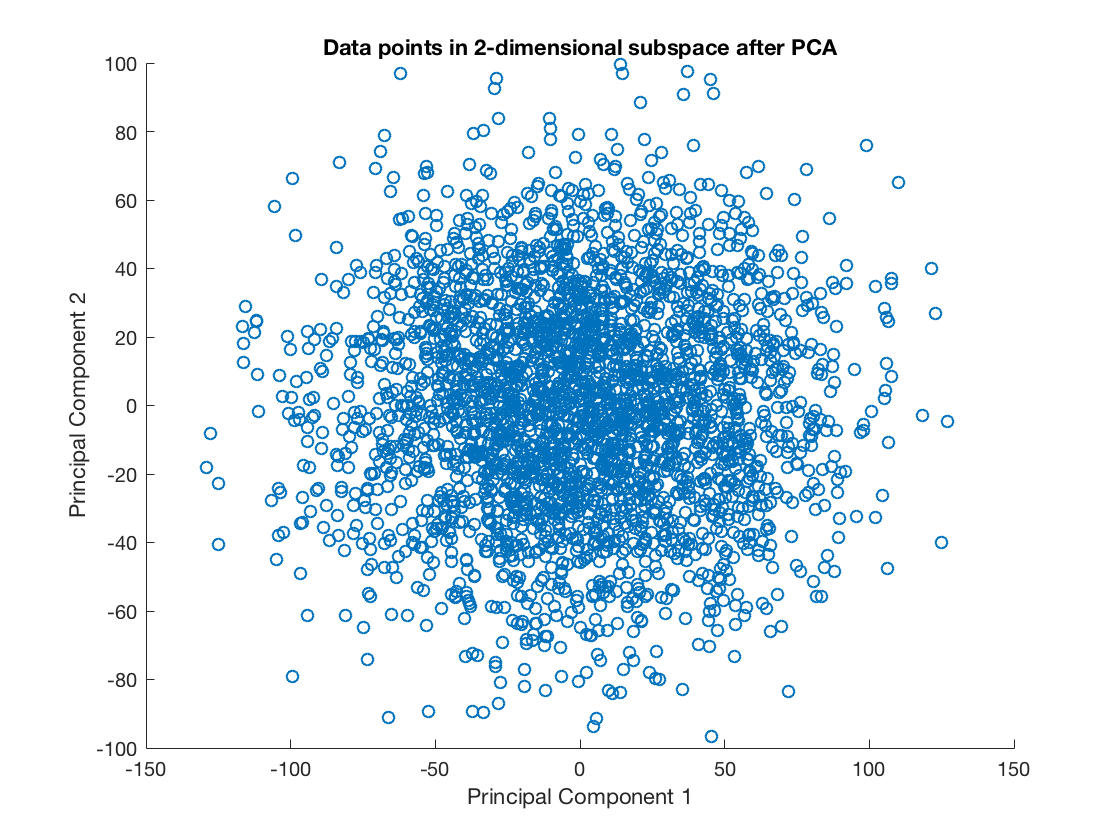
\includegraphics[width=.5\linewidth]{svd.png}
}
\caption{Data points in 2-dimensional subspace after PCA}
\label{fig:name}
\end{figure}
Get the best rank-2 approximation of the SVD which gave me $U'$ as a $3000\times2$ matrix, $S'$ as a $2\times2$ matrix and $V'$ as a $40\times2$. There are two approaches to get the subspace coordinates:
\begin{itemize}
\item $V'$ describes the subspace which minimizes the squared sum of residuals. Use $\mathbf{<A,V'>}$ to get the new coordinates in the 2-dimensional subspace whose axes are the two principal components.
\item $A = USV^T \Rightarrow AV=US$. Use $\mathbf{<U',S'>}$ to get the new coordinates in the 2-dimensional subspace whose axes are the two principal components.
\end{itemize}

\section{Frequent Directions and Random Projections (40 points)}

\paragraph{A (20 points):}
\begin{itemize}
\item How large does $l$ need to be for the above error to be at most $||A||_F^2/10$?
$$||A||_F^2=1.2618\times10^7$$
$$||A||_F^2/10=1.2618\times10^7/10=1.2618\times10^6$$
\begin{table}[H]
\centering
\begin{tabular}{c|c}
l & $\max_{||x||=1}|||A_x||^2-||B_x||^2|$\\
\hline
1 & 5.1367e+06\\
2 & 5.0209e+06\\
3 & 2.8471e+06\\
4 & 1.6867e+06\\
5 & 1.0815e+06\\
\end{tabular}
\end{table}
When $\mathbf{l=5}$, the above error is,
$$\max_{||x||=1}|||A_x||^2-||B_x||^2|=||A^TA-B^TB||=1.0815\times10^6<||A||_F^2/10$$
\item How does this compare to the theoretical bound (e.g. for k = 0).
$$l=k+\frac{1}{\epsilon}=0+\frac{1}{0.1}=10$$
The empirical $l=5$ is less than the theoritical $l=10$.
\item How large does $l$ need to be for the above error to be at most $||A-A_k||_F^2/10$ (for $k=2$)?
$$||A-A_k||_F^2=4.4800\times10^6$$
$$||A-A_k||_F^2/10=4.4800\times10^6/10=4.4800\times10^5$$
\begin{table}[H]
\centering
\begin{tabular}{c|c}
l & $\max_{||x||=1}|||A_x||^2-||B_x||^2|$\\
\hline
1 & 5.1367e+06\\
2 & 5.0209e+06\\
3 & 2.8471e+06\\
4 & 1.6867e+06\\
5 & 1.0815e+06\\
6 & 7.0533e+05\\
7 & 2.1034e+05\\
\end{tabular}
\end{table}
When $\mathbf{l=7}$, the above error is,
$$\max_{||x||=1}|||A_x||^2-||B_x||^2|=||A^TA-B^TB||=2.1034\times10^5<||A-A_k||_F^2/10$$
\end{itemize}

\paragraph{B (20 points):}
$$l=219$$
Since \texttt{Random Sampling} is a random algorithm, we need to specify the probability of failure $\delta$. Assuming we want the probability of failure $\delta=0.01$, then we get $l=219$.\\\\
The experiment is as follows,
\begin{itemize}
\item Initialize $l = 0$
\item Run \texttt{Random Sampling} algorithm for 100 times.
\item If the error bound $||A^TA-B^TB||\le||A-A_k||_F^2/10$ is acheived, record $l$. Otherwise, increment $l$ and run Step2 again. Repeat until the error bound is acheived and record $l$.
\item Run Step1-3 for 100 times and get 100 $l$s. Calculate the mean of the 100 $l$s.
\end{itemize}
According to \textbf{Central Limit Theorem}, the real $\hat{l}$ is equal to the expectation of $l$, which approximately equals the mean of $l$s.

\section{Linear Regression (40 points)}

\paragraph{A (20 points):} X and Y
\begin{table}[H]
\centering
\begin{tabular}{c|c}
Coefficients & $norm(\hat{Y}-Y,2)$\\
\hline
C0.0 & 4.974259 \\ 
C0.1 & 4.974260 \\ 
C0.3 & 4.974400 \\ 
C0.5 & 4.975351 \\ 
C1.0 & 4.991665 \\ 
C2.0 & 5.243593 \\ 
\end{tabular}
\end{table}

\paragraph{B (20 points):} three subsets of X and Y
\begin{table}[H]
\centering
\begin{tabular}{c|c|c|c|c}
Coefficients & X1,Y1 & X2,Y2 & X3,Y3 & Average\\
\hline
C0.0 & 3.254072 & 3.202433 & 3.351705 & 3.269403333 \\
C0.1 & 3.251804 & 3.203395 & 3.350592 & 3.268597 \\
C0.3 & 3.234075 & 3.211249 & 3.341872 & 3.262398667 \\
C0.5 & 3.200887 & 3.227794 & 3.325420 & 3.251367 \\
C1.0 & 3.087773 & 3.319639 & 3.266257 & 3.224556333 \\
C2.0 & 3.366890 & 3.882281 & 3.332971 & 3.527380667 \\
\end{tabular}
\end{table}
Averaging the result of the three subsets, \textbf{Ridge Regression with} $\mathbf{s=1.0}$ works best with $norm(\hat{Y}-Y,2)\approx3.22456$.

\newpage

\section{Appendix: Codes}
\begin{lstlisting}[language=Matlab]
function result = svd_norm(A, U, S, V)
    result = zeros(10,1);
    for k = 1:10
        Ak = U(:,1:k) * S(1:k,1:k) * V(:,1:k)';
        result(k) = norm(A-Ak,2)
    end
end

function k = svd_norm2(A, U, S, V)
    normA = norm(A,2);
    k = 1;
    while 1
        Ak = U(:,1:k) * S(1:k,1:k) * V(:,1:k)';
        sse = norm(A-Ak,2);
        if sse >= 0.1*normA
            k = k+1;
        else
            break
        end
    end
end

function [B] = FD(A,l)
    [n,d] = size(A);

    B = zeros(2*l,d);

    % fill in the rest here
    for i = 1:n
        idx = find(all(B==0,2),1);
        B(idx,:) = A(i,:);
        idx = find(all(B==0,2),1);
        if isempty(idx)
            [U,S,V] = svd(B);
            delta = S(l,l)^2;
            for j = 1:l-1
                S(j,j) = (S(j,j)^2-delta)^0.5;
            end
            for j = l:l*2
                S(j,j) = 0;
            end
            B = S*V';
        end
    end
end

function l = FD_l(A)
    froNorm = norm(A, 'fro')^2
    l = 1;
    while 1
        B = FD(A, l);
        error = norm(A'*A - B'*B, 2)
        if error <= froNorm/10
            break
        end
        l = l + 1;
    end
end

function l = FD_l2(A, k)
    [U,S,V] = svd(A);
    Uk = U(:,1:k);
    Sk = S(1:k,1:k);
    Vk = V(:,1:k);
    Ak = Uk*Sk*Vk';
    froNorm = norm(A-Ak, 'fro')^2
    l = 1;
    while 1
        B = FD(A, l);
        error = norm(A'*A - B'*B, 2)
        if error <= froNorm/10
            break
        end
        l = l + 1;
    end
end

function [B] = RP(A, l)
    [n, d] = size(A);
    S = normrnd(0,1,[l,n])/l^0.5;
    B = S*A;
end

function l = RP_l(A)
    froNorm = norm(A, 'fro')^2
    l = 1;
    while 1
        B = RP(A,l);
        error = norm(A'*A-B'*B, 2);
        if error <= froNorm/10
            break
        end
        l = l + 1;
    end
end

function max = RP_l2(A)
    max = 0;
    for i = 1:100
        l = RP_l(A)
        if (l > max)
            max = l;
        end
    end
end

\end{lstlisting}
\end{document}
